\documentclass[10pt]{article}
\usepackage{icmlko}

\icmlmeta{IP 파운데이션 월드모델}{80}{씨앗 넷이 처음으로 채택을 막았다}{부분집합 마흔다섯 개를 훑어 넷을 검정했고 하나도 안 붙었다 --- 그리고 왜 안 붙는지가 더 중요했다}

\begin{document}

\twocolumn[
\icmlheader

\begin{abstract}
노트 79에서 만화의 3분의 1(AniList 한국 작품)을 빼니 판정치가 $+$0.0088 오르고
반폭이 16\% 줄었다 --- \textbf{도메인을 하나 더한 것과 같은 값}이다. 그런 잡음
부분집합이 다른 도메인에도 있는지 여덟 도메인의 범주형 필드를 전수로 훑었다
--- \textbf{부분집합 45개}. 도메인 안 자기 $\rho$를 크게 올리는 것이 셋
나왔다: 애니 무료작($+$0.0774, 326건), 애니 성인물($+$0.0358), 웹툰 연재중
($+$0.0160). \textbf{그런데 앙상블 자로 검정하니 하나도 안 붙었다.} 최선인
애니 무료작이 $\Delta+$0.0042이고 씨앗 넷 중 \textbf{하나만} 채택이다. 씨앗
하나로 판정했다면 붙였을 것이다 --- \textbf{노트 72의 씨앗 넷 규약이 처음으로
실제로 무언가를 막았다.} 왜 안 붙는지가 더 중요하다. \textbf{자기 상관 이득이
판정치로 거의 안 옮겨간다} --- 애니 무료작은 자기 $\rho$를 $+$0.077 올리는데
판정치는 $+$0.004, 즉 \textbf{18분의 1}이다. 노트 74 · 78의 법칙($r\approx+$0.99)은
\emph{도메인 사이}의 관계이지 \emph{한 도메인 안}의 처방에는 안 통한다. 노트
79의 만화가 통과한 것은 부분집합이 더 크고(3분의 1) 더 극단적으로 잡음이었기
때문이다(자기 $\rho$ $+$0.083).
\end{abstract}
]

\begin{figure*}[t]
\centering
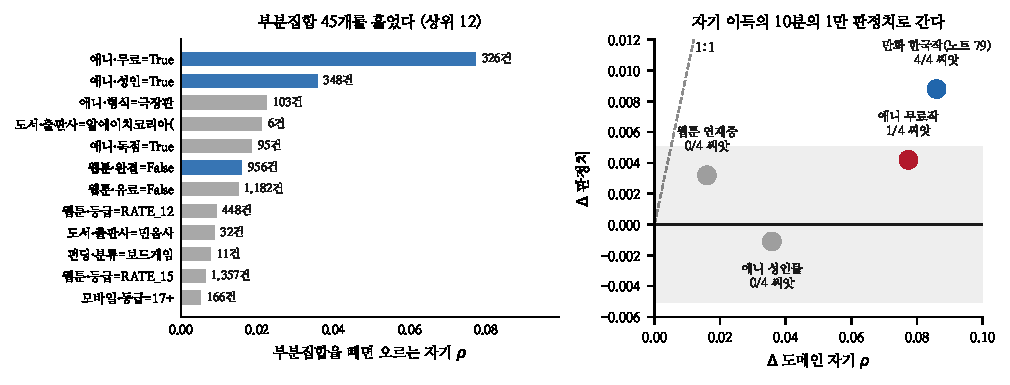
\includegraphics[width=\textwidth]{figs/seeds.pdf}
\caption{왼쪽 --- 부분집합 45개 중 상위 12(파랑이 검정한 것). 오른쪽 ---
자기 이득과 판정치 이득.}
\end{figure*}

\section{마흔다섯 개를 훑었다}

절차를 둘로 나눴다. \textbf{선별}은 도메인 안 자기 순위 상관만 쓴다 ---
부분집합을 빼고 다시 재서 오르는가. 한 도메인 안 교차검증이라 싸다(노트 37).
\textbf{판정}은 선별에서 올라온 것만 앙상블 자로 짝지은 붓스트랩 $+$ 씨앗 넷.

\begin{table}[t]
\centering\tsize
\caption{빼면 자기 $\rho$가 오르는 상위 여섯.}
\begin{tabular}{llrr}
\toprule
도메인 & 부분집합 & 건수 & $\Delta$자기 \\
\midrule
\textbf{애니} & \textbf{무료 제공작} & 326 & \textbf{$+$0.0774} \\
애니 & 성인물 & 348 & $+$0.0358 \\
애니 & 극장판 & 103 & $+$0.0225 \\
애니 & 독점작 & 95 & $+$0.0186 \\
웹툰 & 연재중 & 956 & $+$0.0160 \\
웹툰 & 무료작 & 1182 & $+$0.0150 \\
\bottomrule
\end{tabular}
\end{table}

의미 근거가 있는 셋을 골라 검정했다. 무료 제공작은 구독 없이 보는 것이라
반응이 다른 경로로 생기고, 성인물은 별도 카테고리이며, 연재중 작품은 축(연재
밀도)과 라벨(관심 수)이 둘 다 아직 자란다.

\section{하나도 안 붙었다}

\begin{table}[t]
\centering\tsize
\caption{채택 검정. 앙상블 자, 붓스트랩 120회, 씨앗 넷.}
\begin{tabular}{lrr}
\toprule
& $\Delta$판정치 & 채택 씨앗 \\
\midrule
애니 무료작 제외 & $+$0.0042 & \textbf{1/4} \\
웹툰 연재중 제외 & $+$0.0032 & 0/4 \\
애니 성인물 제외 & $-$0.0011 & 0/4 \\
애니 무료$+$성인 제외 & $+$0.0042 & 1/4 \\
\midrule
\multicolumn{2}{l}{(참고) 만화 한국작 제외, 노트 79} & 4/4 \\
\bottomrule
\end{tabular}
\end{table}

애니 무료작의 첫 씨앗이 $[+$0.0003, $+$0.0098$]$로 아슬아슬하게 0을 넘는다.
\textbf{씨앗 하나로 판정했다면 붙였을 것이다.} 나머지 셋은 전부 0을 포함한다.

\claimx{노트 72의 씨앗 넷 규약이 처음으로 실제 채택을 막았다. 그 규약은 노트
67(작은 표본에서 고른 배선이 큰 표본에서 사라진다)의 교훈으로 만들었고, 만든
뒤 여덟 노트 동안 아무것도 안 막다가 여기서 걸렸다.}{씨앗 넷도 임의의 수다.
같은 데이터에서 뽑으므로 표본 자체의 편향은 못 잡는다 --- 넷이 다 통과해도
표본이 바뀌면 사라질 수 있다(노트 67이 그 사례다).}

\section{왜 안 붙나 --- 자기 이득이 안 옮겨간다}

\begin{table}[t]
\centering\tsize
\caption{처방 전후. 애니와 웹툰.}
\begin{tabular}{lrrrr}
\toprule
& 자기 $\rho$ & 대상 & 출처 & 판정치 \\
\midrule
애니 현행 & $+$0.291 & $+$0.258 & $+$0.333 & $+$0.4003 \\
애니 무료 제외 & \textbf{$+$0.369} & $+$0.291 & $+$0.347 & $+$0.4045 \\
\midrule
웹툰 현행 & $+$0.480 & $+$0.455 & $+$0.379 & $+$0.4003 \\
웹툰 완결만 & $+$0.496 & $+$0.469 & $+$0.390 & $+$0.4035 \\
\bottomrule
\end{tabular}
\end{table}

애니 무료작을 빼면 자기 $\rho$가 $+$0.077 오르는데 판정치는 $+$0.004다.
\textbf{18분의 1만 옮겨간다.}

\claimx{노트 74 · 78의 법칙($r\approx+$0.99, 자기 $\rho$가 대상 전이를 결정한다)은
\emph{도메인 사이}의 관계다. \emph{한 도메인 안}에서 표본을 바꿔 자기 $\rho$를
올려도 그만큼 전이가 오르지 않는다 --- 애니에서 이득의 44\%만 대상 전이로
갔고, 판정치로는 여덟 도메인에 희석돼 18분의 1이 됐다.}{노트 79의 만화는 자기
$+$0.086 중 86\%가 대상 전이로 갔다. 도메인마다 다르고 무엇이 비율을 정하는지
모른다.}

\begin{quote}\fontsize{9.5}{11.5}\selectfont
\textbf{산술이 단순하다.} 판정치는 아홉 대상의 평균이고 한 도메인의 처방은
그 도메인이 대상인 한 자리에만 온전히 들어간다. 자기 이득의 절반이 대상
전이로 가고 그것이 다시 9로 나뉘면 $0.077\times0.44/9=0.0038$ --- 관측된
$+$0.0042와 맞는다.
\end{quote}

\section{한계}

\begin{itemize}[leftmargin=1.1em,itemsep=0.15em]
\item 범주형 필드만 훑었다. 연속값(가격대 · 연도대 · 표본 크기)으로 자르면
      다른 부분집합이 나올 수 있다.
\item 부분집합 45개를 보고 상위 넷을 검정했다. 선택 편향이 크고, 그래서 씨앗
      넷을 요구한 것이다.
\item ``의미 근거''로 셋을 골랐는데 그 판단은 내가 했다. 극장판 · 독점작은
      근거를 못 대서 뺐다.
\item 자기 이득이 대상 전이로 가는 비율(애니 44\%, 만화 86\%)이 왜 다른지
      모른다.
\item 애니 무료작 제외가 1/4로 아깝다. 붓스트랩을 300회로 올리면 달라질 수
      있는데 안 했다.
\end{itemize}

\section{다음}

\begin{enumerate}[leftmargin=1.3em,itemsep=0.15em]
\item 자기 이득이 전이로 가는 비율을 결정하는 것이 무엇인지 --- 부분집합 크기?
      도메인의 축 수? 여러 사례를 모아 본다.
\item 연속값으로 자른 부분집합을 훑는다.
\item 열째 도메인 --- 노트 79 뒤 반폭이 0.0339이고 셀 70$\to$90이면 0.0300이다.
\item 팝업 라벨의 신뢰도(노트 79의 숙제). 같은 팝업을 두 번 잰 자료가 있는지.
\end{enumerate}

\vspace{0.6em}
\hrule height 0.3pt
\vspace{0.5em}
{\footnotesize
\textbf{참고문헌}\\[0.3em]
Cawley, G. C., Talbot, N. L. C. (2010). On over-fitting in model selection and
subsequent selection bias in performance evaluation. \emph{JMLR}, 11, 2079--2107.\\[0.15em]
Ioannidis, J. P. A. (2005). Why most published research findings are false.
\emph{PLoS Medicine}, 2(8), e124.\\[0.15em]
Bouthillier, X. et al. (2021). Accounting for variance in machine learning
benchmarks. \emph{MLSys}, 3, 747--769.\\[0.15em]
Ben-David, S. et al. (2010). A theory of learning from different domains.
\emph{Machine Learning}, 79(1--2), 151--175.\\[0.15em]
Efron, B., Tibshirani, R. J. (1993). \emph{An Introduction to the Bootstrap}.
Chapman \& Hall.
}

\end{document}
